% Created 2020-10-26 Mon 12:48
% Intended LaTeX compiler: pdflatex
\documentclass[11pt]{article}
\usepackage[utf8]{inputenc}
\usepackage[T1]{fontenc}
\usepackage{graphicx}
\usepackage{grffile}
\usepackage{longtable}
\usepackage{wrapfig}
\usepackage{rotating}
\usepackage[normalem]{ulem}
\usepackage{amsmath}
\usepackage{textcomp}
\usepackage{amssymb}
\usepackage{capt-of}
\usepackage{hyperref}
\usepackage[english]{babel}
\usepackage[T2A]{fontenc}
\usepackage[utf8]{inputenc}
\usepackage{minted}
\usepackage{wrapfig}
\author{Макаров Сергей, группа 427}
\date{\today}
\title{Контрольная работа №3}
\hypersetup{
 pdfauthor={Макаров Сергей, группа 427},
 pdftitle={Контрольная работа №3},
 pdfkeywords={},
 pdfsubject={},
 pdfcreator={Emacs 27.1 (Org mode 9.3)}, 
 pdflang={English}}
\begin{document}

\maketitle

\section{Задача}
\label{sec:org442a6ab}
Построить границы доминирования для приводимого CFG:
\begin{center}
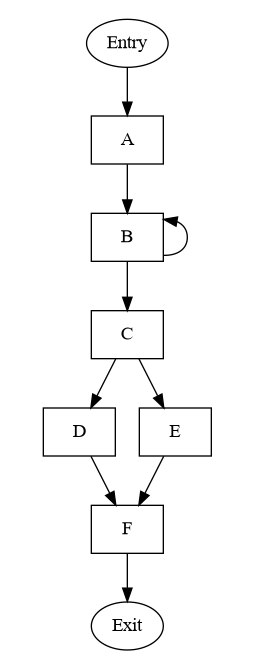
\includegraphics[height=200px]{cfg3.png}
\end{center}
\subsection{Решение}
\label{sec:orge53e9bf}
Построим дерево доминаторов для CFG. Для этого воспользуемся DFA:
\begin{gather*}
Out[B] = In[B] \cup \{B\} \\
\wedge = \cap
\end{gather*}

\begin{gather*}
D(Entry) = \{Entry\} \\
D(A) = \{A\} \cup D(Entry) = \{A, Entry\} \\
D(B) = \{B\} \cup (D(B) \cap D(A)) = \{A, B\} \\
D(C) = \{C\} \cup (D(B)) = \{A, B, C\} \\
D(D) = \{D\} \cup D(C) = \{A, B, C, D\} \\
D(E) = \{E\} \cup D(C) = \{A, B, C, E\} \\
D(F) = \{F\} \cup (D(D) \cap D(E)) = \{A, B, C, F\} \\
D(Exit) = \{Exit\} \cup D(F) = \{F, Exit\}
\end{gather*}
Таким образом,
\begin{gather*}
Idom(Entry) = \emptyset, Idom(A) = Entry, Idom(B) = A, Idom(C) = B \\
Idom(D) = C, Idom(E) = C, Idom(F) = C, Idom(Exit) = F.
\end{gather*}
Получаем дерево доминаторов:
\begin{center}
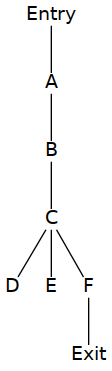
\includegraphics[height=200px]{dom-tree2.png}
\end{center}

Вычислим теперь границы доминирования. В заданном CFG две точки сбора: B и F. Рассмотрим
каждую из них.
\begin{equation*}
Pred(B) = \{A, B\}
\end{equation*}
Проходя по дереву доминаторов от $A$ и $B$ до $Idom(B) = A$ заключаем, что $B \in DF(B)$.
\begin{equation*}
Pred(F) = \{D, E\}
\end{equation*}
Проходя по дереву доминаторов от $D$ и $E$ до $Idom(F) = C$ заключаем, что $F \in DF(D), DF(E)$.
Границы доминирования остальных блоков пусты. В самом деле, блоки $A$ и $Entry$ доминируют над
всеми, поэтому их границы доминирования пусты. Блок $C$ доминирует над всеми блоками ниже, поэтому
его граница доминирования также пуста. Аналогично, $DF(F) = \emptyset$.
\end{document}
